% This document is used for Daya Bay MACRO PMT pressure test report


\documentclass{beamer}
\usepackage{graphicx}

%\setlength{\unitlength}{\textwidth}

\setbeamertemplate{navigation symbols}{}
\setbeamertemplate{footline}[page number]
\setbeamertemplate{caption}[numbered]
%\setbeamerfont{purisa}
\usetheme{default}
\logo{
\includegraphics[height=1cm]{Dyb_logo.png}}
\begin{document}
\title{Status of MACRO PMT pressure tests at SAB}
\author{Logan Lebanowski, Shih-Kai Lin}
%\institute{University of Houston}
\date{Sep 23, 2010}

\begin{frame}
\begin{center}
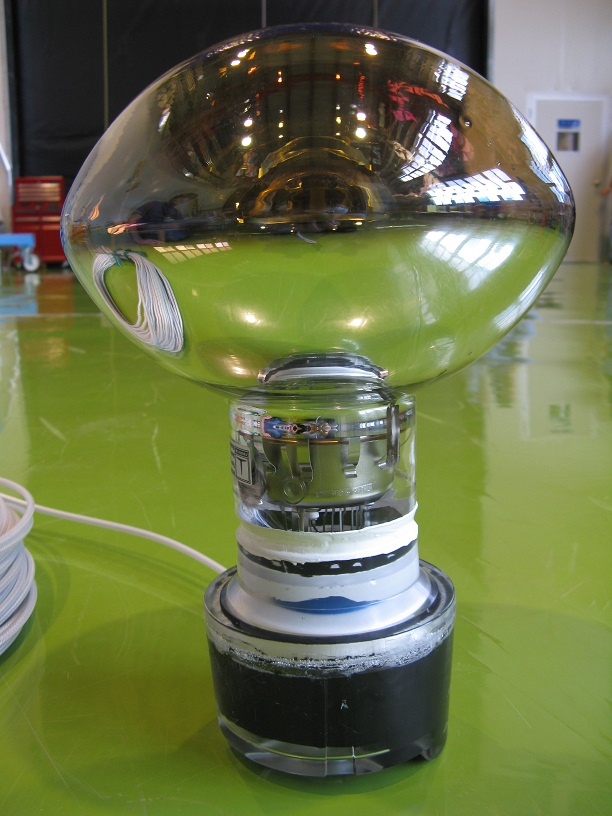
\includegraphics[height=4cm]{IMG_1048.jpg}
\end{center}
\titlepage
\end{frame}


\begin{frame}{pressure test results}
\begin{itemize}
	\item As of September 23, we have passed 47 of 50 PMTs.
	\item 11 PMTs were tested during the past week (September 16 - September 22). PMT 8870
	had a hole in the cable jacket. It was fixed and tested again.
\end{itemize}
\begin{table}
\small
\begin{tabular}{c|c|c|c|c}
%\setlength{\tabcolsep}{2pt}
	SN & mass (g) & pressure (psig) & test time (h:m) & result \\
	\hline
	7851 & 564 & 12.1 & 14:48 & PASS$^1$ \\
	7127 & 582 & 12.2 & 8:51 & PASS$^2$ \\
	7820 & 595.5 & 12.0 & 14:44 & PASS$^3$ \\
	7267 & 643.5 & 12.0 & 8:44 & PASS$^2$ \\
	7934 & 609 & 12.0 & 14:48 & FAIL$^4$ \\
	8430 & 554 & 12.0 & 47:23 & FAIL$^5$ \\
	8870 & 587.5 & 12.0 & 7:27 & PASS$^2$ \\
	7899 & 566 & 12.0 & 16:24 & PASS$^3$ \\
	7765 & 573 & 12.1 & 7:05 & PASS$^3$ \\
	7471 & 601 & 12.0 & 14:56 & PASS$^1$ \\
	6873 & 601.5 & 12.2 & 8:20 & PASS$^1$ \\
\end{tabular}
\caption {pressure test result: For PASS/FAIL reasons, please see the table in the next slide.}
\end{table}
%\begin{itemize}
%	\item For PASS/FAIL reasons, please see the table in the next slide.
%\end{itemize}
\end{frame}

\begin{frame}{PASS/FAIL reasons}
	\setlength{\tabcolsep}{2pt}
	\small
	\begin{table}
		\begin{tabular}{|c|p{3.5in}|}
		\hline
		\textbf{number} & \textbf{reason} \\
		\hline
		\hline
		1 & Cable dry. No leaks or cracks. \\
		\hline
		2 & 1+Some water penetrated the mastic tape seal of the cable strain relief plug,
			but did not penetrate the UW cable plug. \\
		\hline
		3 & Moisture on the SHV end in the sealing tube. Conductivity test performed. \\
		\hline
		4 & Acrylic cap contains much water.(see photo) \\
		\hline
		5 & A big crack and a little hole in the PMT. Photocathode was gone.(see photo) \\
		\hline
		\end{tabular}
	\caption{PASS/FAIL reasons}
	\end{table}
\end{frame}

\begin{frame}{photos: PMT 7934}
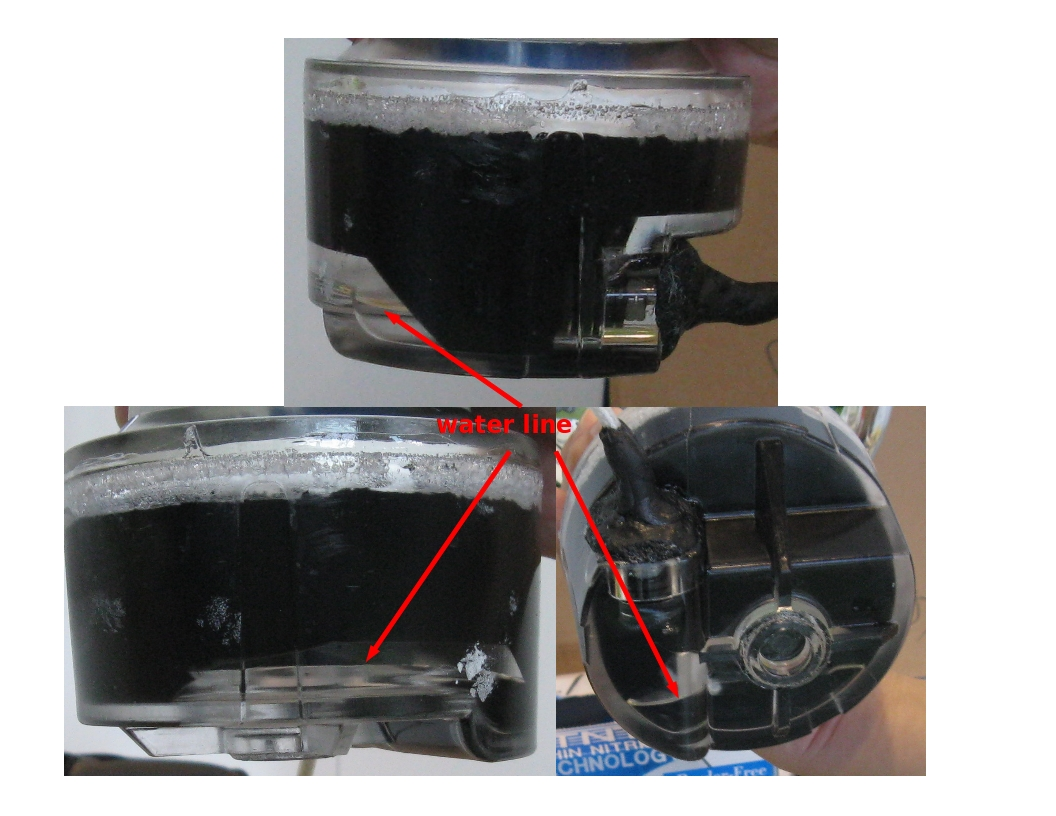
\includegraphics[width=12cm]{PMT7934.jpg}
\end{frame}


\begin{frame}{photos: PMT 8430}
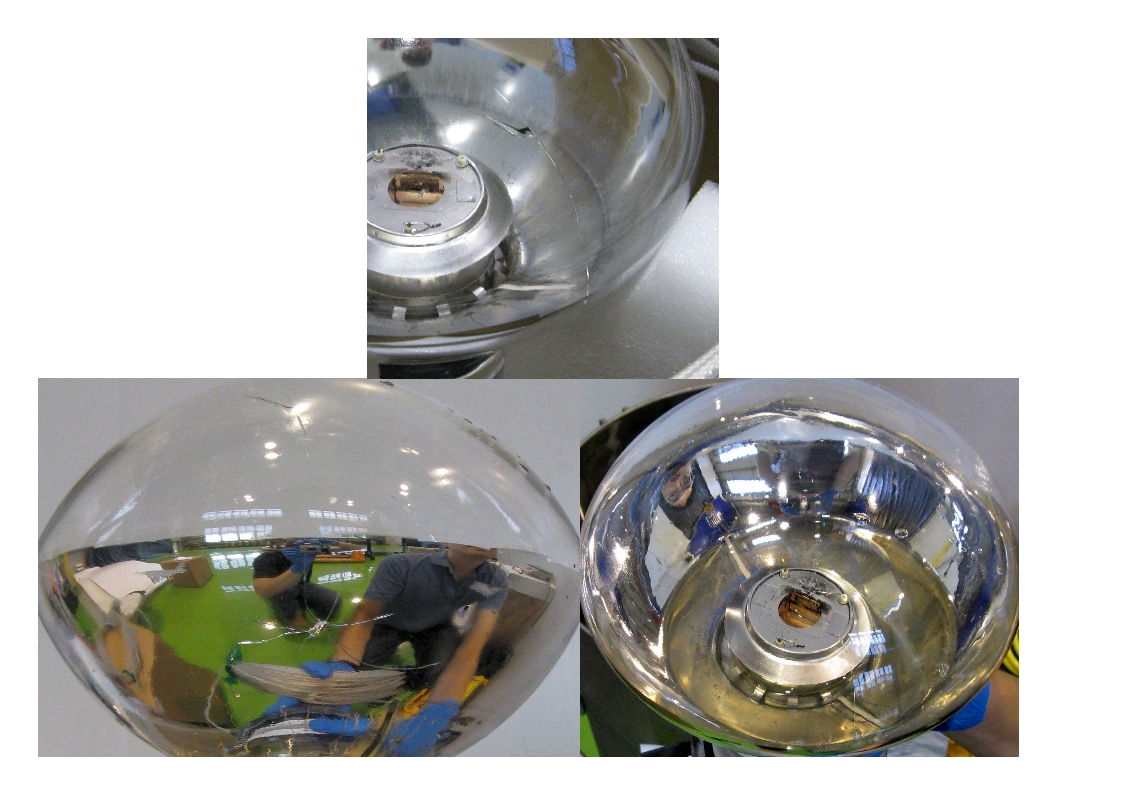
\includegraphics[width=12cm]{PMT8430.jpg}
\end{frame}

\begin{frame}{signal test results}
	\setlength{\tabcolsep}{2pt}
	\small
	\begin{center}
	\begin{tabular}{|l|p{1.2cm}|p{1.9cm}|p{1.5cm}|p{1.7cm}|}
		\hline
		\textbf{SN}&\textbf{Rate (kHz)}&\textbf{DGUT rate (kHz)}&\textbf{Rise time (ns)}&
		\textbf{DGUT rise time (ns)}\\
		\hline
		\hline
		6494&9.5&0.84&4.8&5.5\\
		7357&5.0&0.45&4.8&7.4\\
		6238&2.0&0.45&6.1&5.2\\
		7278&3.0&0.38&5.2&7.5\\
		7945&1.8&0.5&5.6&5.7\\
		7379&1.5&0.63&5.0&5.3\\
		8356&5.0&1.21&5.5&5.9\\
		7520&9.0&0.37&5.0&4.8\\
		7343&4.3&0.7&5.0&4.4\\
		8756&5.0&0.56&4.5&4.5\\
		\hline
	\end{tabular}
	\end{center}
\end{frame}

\begin{frame}{signal test results (cont.)}
	\setlength{\tabcolsep}{2pt}
	\small
	\begin{center}
	\begin{tabular}{|l|p{1.2cm}|p{1.9cm}|p{1.5cm}|p{1.7cm}|}
		\hline
		\textbf{SN}&\textbf{Rate (kHz)}&\textbf{DGUT rate (kHz)}&\textbf{Rise time (ns)}&
		\textbf{DGUT rise time (ns)}\\
		\hline
		\hline
		7692&2.3&0.41&5.8&5.6\\
		8870&10.0&4.42&5.1&3.6\\
		8901&4.0&0.89&5.1&6.4\\
		6659&2.4&0.58&7.3&5.4\\
		6432&20.0&3.04&5.0&5.5\\
		7851&1.5&1.08&5.4&6.0\\
		7127&9.0&0.84&4.3&4.4\\
		7820&7.0&0.49&4.9&5.8\\
		7267&12.0&3.58&4.9&4.1\\
		\hline
	\end{tabular}
	\end{center}
\end{frame}



\end{document}

